\documentclass[11pt, english]{article}
\usepackage[english]{babel}
\usepackage[utf8]{inputenc}



\usepackage{geometry}
 \geometry{
 a4paper,
 left=20mm,
 top=30mm,
 right=20mm
 }


\usepackage{listings}
\usepackage{amsmath}
\usepackage{amsfonts}
\usepackage{amssymb}
\usepackage{amsthm} 
\usepackage{mathrsfs}
\usepackage{mathabx}
\usepackage{graphicx}
\usepackage{eurosym}
\usepackage{subfigure}
\usepackage{dsfont}
\usepackage{bbm}

%\lstdefinestyle{myCustomMatlabStyle}{
%	language=Matlab,
%	numbers=left,
%	stepnumber=1,
%	numbersep=10pt,
%	tabsize=4,
%	showspaces=false,
%	showstringspaces=false
%}

\usepackage{graphicx} 
\usepackage{fancyvrb} 
\usepackage{listings} 
\usepackage{listings}
\usepackage{amsmath}
\usepackage{amsfonts}
\usepackage{amssymb}
\usepackage{amsthm} 
\usepackage{mathrsfs}
\usepackage{mathabx}
\usepackage{graphicx}
\usepackage{eurosym}
\usepackage{subfigure}
\usepackage{dsfont}
\usepackage{bbm}
\usepackage{inputenc}

\lstdefinestyle{myCustomMatlabStyle2}{% setup listings 
	language=R,% set programming language 
	basicstyle=\small,% basic font style 
	keywordstyle=\bfseries,% keyword style 
	commentstyle=\ttfamily\itshape,% comment style 
	numbers=left,% display line numbers on the left side 
	numberstyle=\scriptsize,% use small line numbers 
	numbersep=10pt,% space between line numbers and code 
	tabsize=3,% sizes of tabs 
	showstringspaces=false,% do not replace spaces in strings by a certain character 
	captionpos=b,% positioning of the caption below 
	breaklines=true,% automatic line breaking 
	escapeinside={(*}{*)},% escaping to LaTeX 
	fancyvrb=true,% verbatim code is typset by listings 
	extendedchars=false,% prohibit extended chars (chars of codes 128--255) 
	literate={"}{{\texttt{"}}}1{<-}{{$\leftarrow$}}1{<<-}{{$\twoheadleftarrow$}}1 
	{~}{{$\sim$}}1{<=}{{$\le$}}1{>=}{{$\ge$}}1{!=}{{$\neq$}}1{^}{{$^\wedge$}}1,% item to replace, text, length of chars 
	alsoletter={.<-},% becomes a letter 
	alsoother={$},% becomes other 
	otherkeywords={!=, ~, $, *, \&, \%/\%, \%*\%, \%\%, <-, <<-, /},% other keywords 
	deletekeywords={c}% remove keywords 
}

\newcommand{\grafico}[5]{
\begin{figure}
[h!tbp]
\centering
\includegraphics[scale=#2, angle=#3]{#1}
%\captionsetup{width=13cm}
\caption{#4\label{#5}}
\end{figure}
}

\newcommand{\su}[2]{\sum\limits_{#1}^{#2}}


\setlength{\parindent}{0pt}

\title{Stochastic Models and Optimization: Problem Set 2}
\author{Roger Garriga Calleja, José Fernando Moreno Gutiérrez, David Rosenfeld, Katrina Walker}
\date{\today}

\begin{document}
\maketitle
\textbf{Problem 1 (Shortest Path using DP):}
\\
\begin{align*}
J_K(i) &= min[a_{ij} + J_{k+1}(j)]\\
K & = 0, 1,...,N-2\\
j & = 1,....,N \\
J_{N-1}(i) & = a_{it}, i = 1, 2,...N \\
J_{K}(i)& = \textup{optimal cost of getting from i to t in N-k moves} 
\end{align*}
\begin{center}
\begin{figure}[h]\small
	\centering
	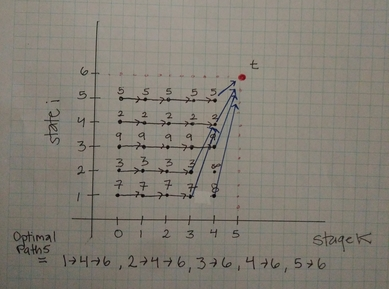
\includegraphics[width=0.7\linewidth]{../../../../../../Desktop/DP_graph}
\end{figure}
\end{center}
\clearpage
\textbf{Problem 2 (Shortest Path via Label Correcting Methods):}
\begin{table}[h]\small
	\centering
	\caption{Bellman Ford Algorithm}
	\label{my-label}
	\begin{tabular}{llll}
		\hline
		Iteration & Exiting Open & Open at end of Iteration & Upper \\ \hline
		0 & - & 1 & $\infty$ \\ \hline
		1 & 1 & 1-2 (2), 1-3(1) & $\infty$ \\ \hline
		2 & 1-2 & 1-3(1), 1-2-4(3) & 2 \\ \hline
		3 & 1-3 & 1-2-4(3) & 2 \\ \hline
		4 & 1-2-4 & 0 & 2 \\ \hline
	\end{tabular}
	\centering
	\caption{Dijkstra’s Algorithm}
	\label{my-label}
	\begin{tabular}{llll}
		\hline
		Iteration & Exiting Open & Open at end of Iteration & Upper \\ \hline
		0 & - & 1 & $\infty$ \\ \hline
		1 & 1 & 1-2 (2), 1-3(1) & $\infty$ \\ \hline
		2 & 1-3 & 1-2(2),  1-3-4(4) & $\infty$ \\ \hline
		3 & 1-2 & 1-3-4(4), 1-2-4(3) & 2 \\ \hline
		4 & 1-2-4 & 1-3-4(4) & 2 \\ \hline
		5 & 1-3-4 & 0 & 2 \\ \hline
	\end{tabular}
\end{table}

\textbf{Problem 3. Clustering:} \textit{We have a set of $N$ objects, denoted $1, 2, . . . , N$, which we want to group in clusters that consist of consecutive objects. For each cluster $i, i + 1, . . . , j$, there is an associated cost $a_{ij}$. We want to find a grouping of the objects in clusters such that the total cost is minimum. Formulate the problem as a shortest path problem, and write a DP algorithm for its solution.}\\

The primitives of the problem are:\\
$x_k$ is the last node of a cluster, with $x_k \in S = {0, 1, ..., N}$ for $k = 0, 1, ..., N$\\
$u_k$ is the decision made at every step k over all objects i such that $i \geq x$.\\
$a_{ij}$ is the cost of a cluster running from i to j.\\
Dynamics:\\
$x_{k+1} = u_k$ and\\
$x_0 = 0$\\
$u_k \in U_k(x) = {i \in S | i\geq x}$ if $x \neq N$ for $k = 0, 1, ..., N-1$ and\\
$u_k \in U_k(x) = {N}$ if $x= N$\\
\\
$g_k(x, u) = a_{x+1,u}$ if $x \neq N$ for $k = 0, 1, ..., N-1$, and \\
$g_k(x, u) = 0$ if $x = N$\\
\\
We then set up the DP algorithm as follows:\\
$J_N(N) = 0$\\
$J_k(i) = \displaystyle \min_{j \in S|j \geq i}[a_{i+1,j} + J_{k+1}(j)]$ if $x \neq N$ and for $k = 0, 1, ..., N-1$\\
$J_k(i) = 0$ if $i = N$\\
Return $J_0(0)$ as the lowest cost.\\


\textbf{Problem 4 (Path Bottleneck Problem):}\textit{ Consider the framework of the shortest path problem. For any path $P$, define the \textbf{bottleneck} arc of $P$ as an arc that has maximum length over all arcs of $P$. We wish to find a path whose length of bottleneck arc is minimum, among all paths connecting the origin node to the destination node. Develop and justify an analog of the label correcting algorithm that solves this problem. }




\textbf{Problem 5. TSP Computational Assignment:}\\\textit{ Visit the website: http://www.math.uwaterloo.ca/tsp/world/countries.html.
Solve the Traveling Salesman Problem for Uruguay based on the dataset provided. You can use your favorite programming language and solution method for the TSP. Provide a printout of your code with detailed documentation, and compare the optimal solution you obtain to the one available at the website.}\\

The code has been done in R. We used 3 heuristic approaches to find approximate the problem: The nearest neighbor, the greedy algorithm and the simulation anneling. We can see that the best approach (anneling) is above the optimal solution by 12\%, however comparing to the second best it just 1\% below. Furthermore, this 1\% represented an important loose in terms of efficiency. In the following table you can see some important results:

\begin{table}[ht]
	\centering
	\begin{tabular}{rrrrr}
		\hline
		& \textbf{optimal} & \textbf{nearest neighbor} & \textbf{greedy} & \textbf{anneling} \\ 
		\hline
		\textbf{distance} & 79114.00 & 100056.45 & 89559.29 & 88985.51 \\ 
		\textbf{distance/optimal} &  & 1.26 & 1.13 & 1.12 \\ 
		\textbf{run time (min)} &  & 0.19 & 2.55 & 11.69 \\ 
		\hline
	\end{tabular}
\end{table}

\lstset{style=myCustomMatlabStyle2}

\lstinputlisting[language=R]{TSP.R}

\end{document}